
\section{Introduction}
The goal of this experiment is to use data-driven model reference control to design an analog controller for a CT system. The open loop system is shown in figure \ref{fig:WH_OL}. It is a Wiener-Hammerstein system. This is a system that consists of a series connection of 2 LTI systems with a nonlinear static system in between them.

\begin{figure}[H]
    \centering
    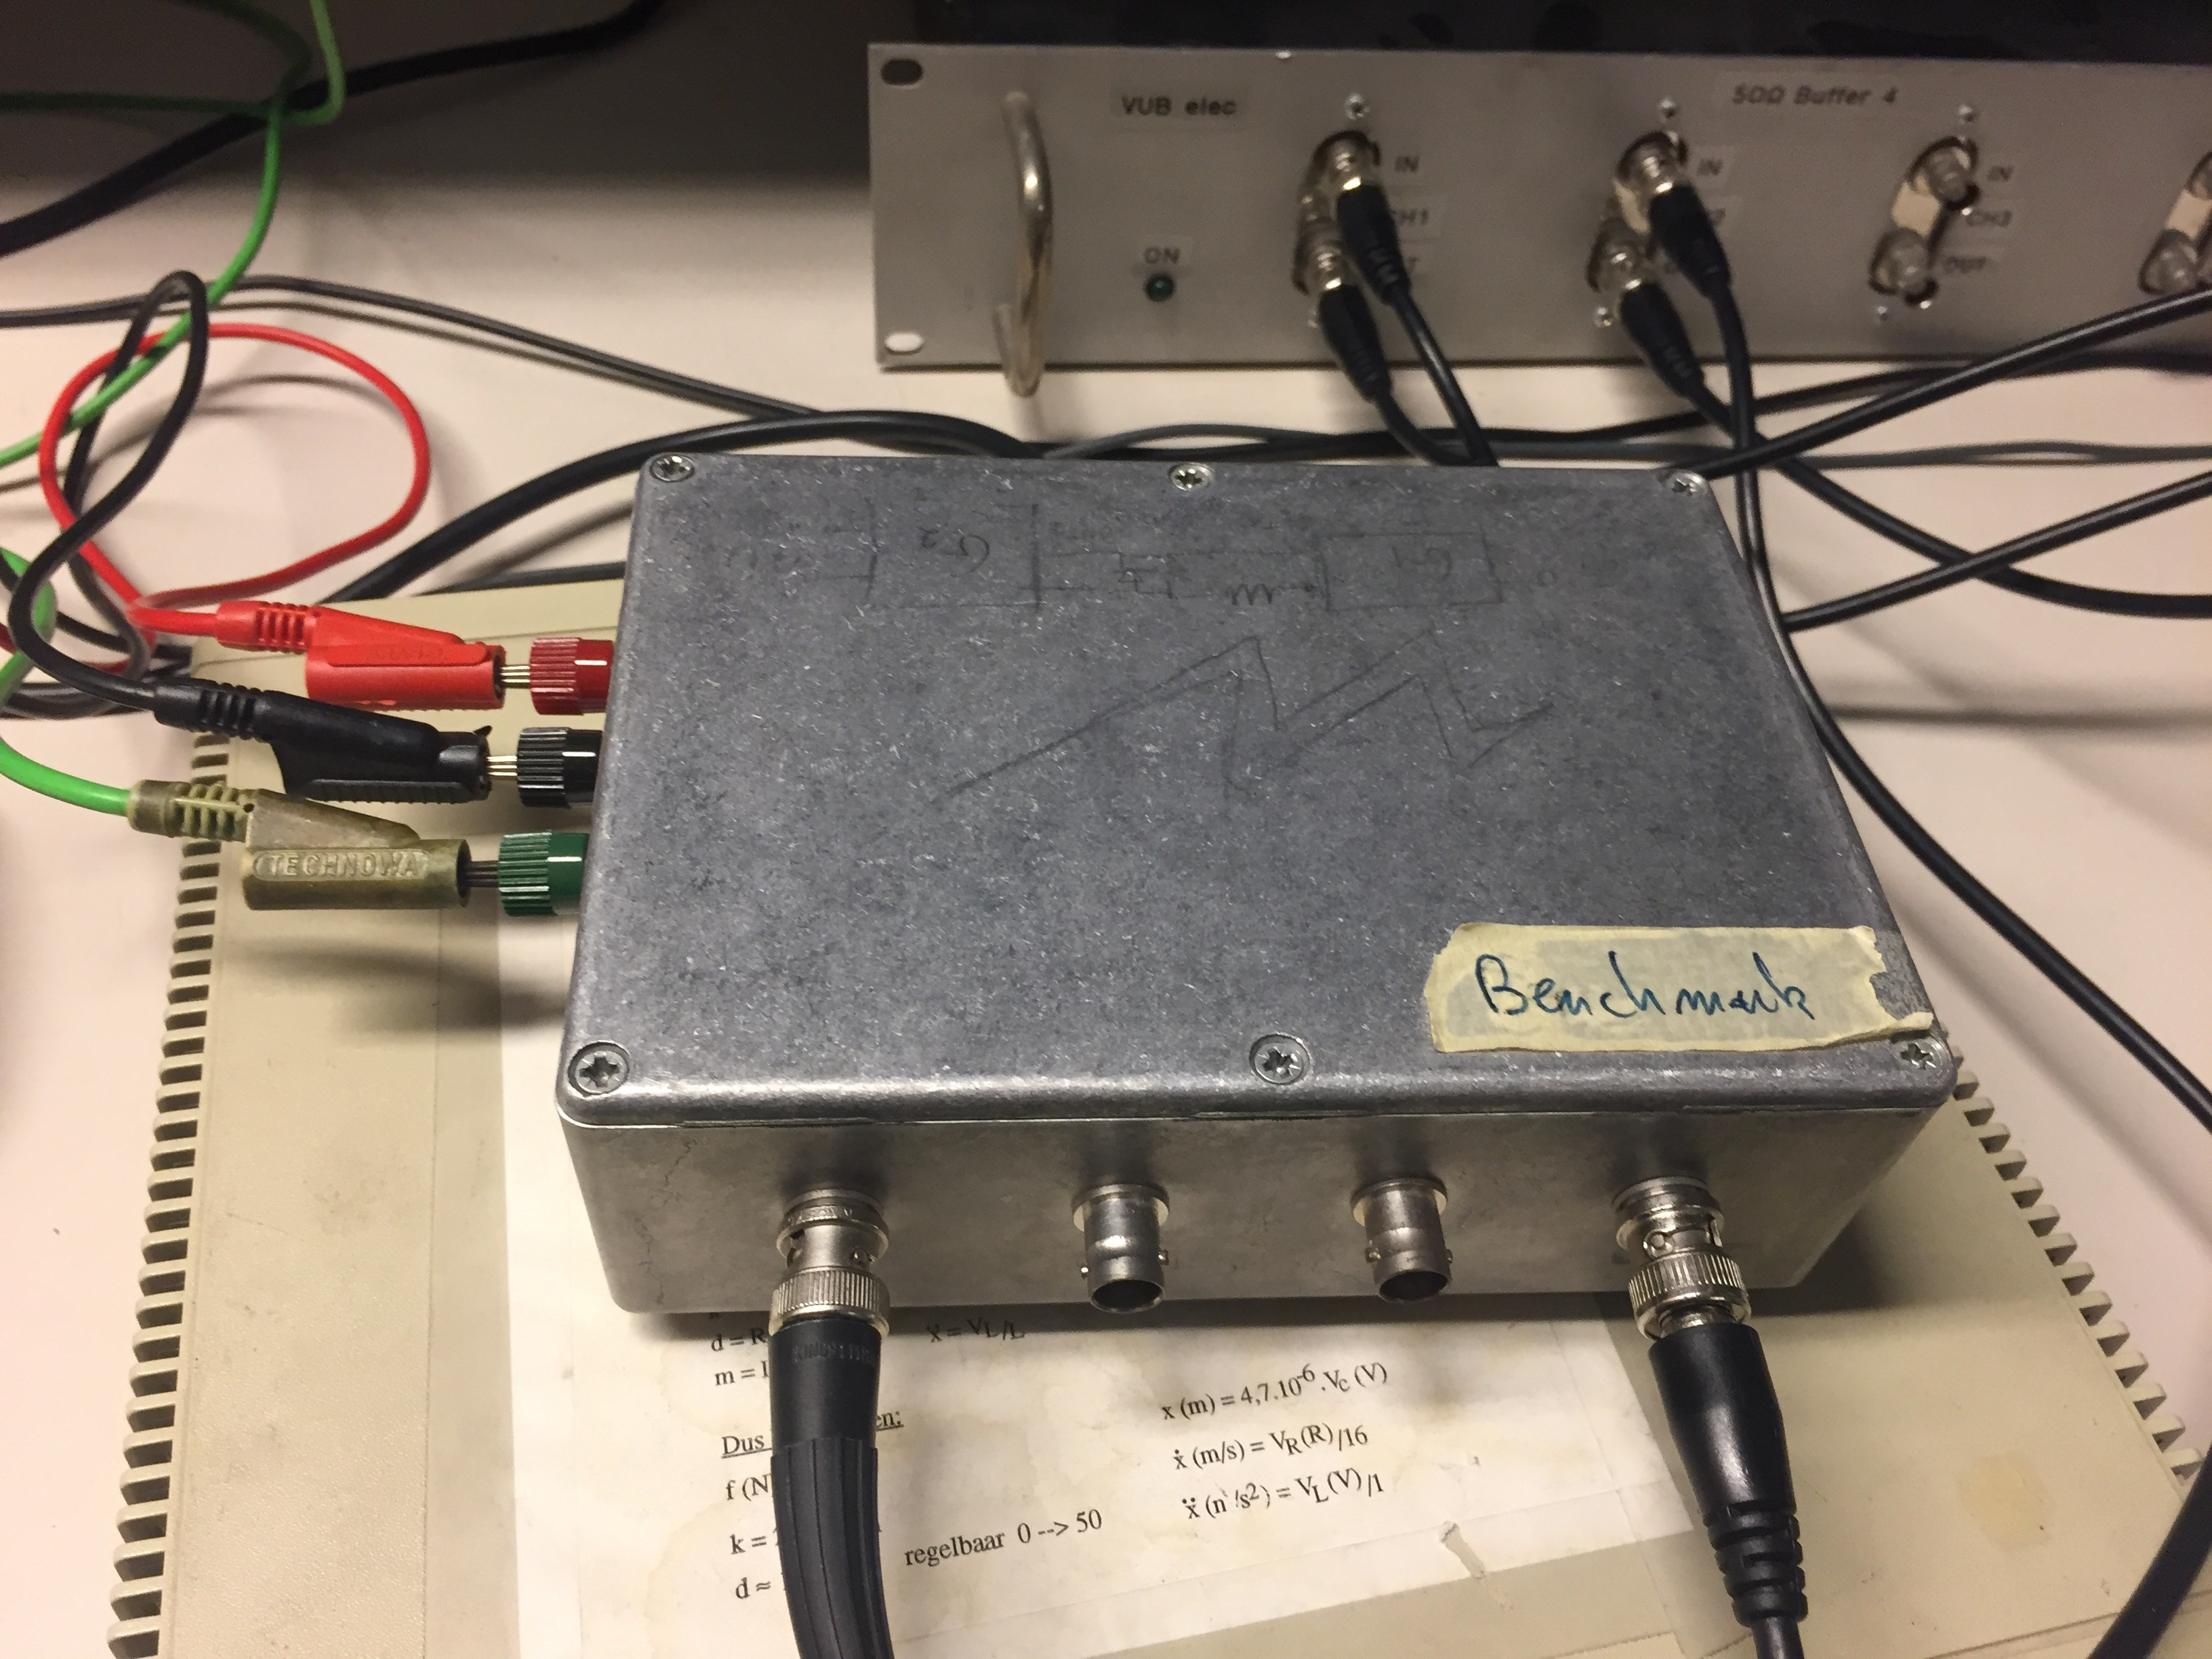
\includegraphics[width = 0.5\textwidth]{figures/DUT.jpg}
    \caption{Picture of the Wiener-Hammerstein system.}
    \label{fig:WH_OL}
\end{figure}


A diagram of the measurement set-up is shown in figure \ref{fig:set-up}. This measurement set-up is a band-limited set-up (section \ref{sec:band-limited}). The device-under-test (DUT) can be the Wiener-Hammerstein system $G(s)$, the controller $K(s)$ or the closed loop system.

\begin{figure}[H]
    \centering
    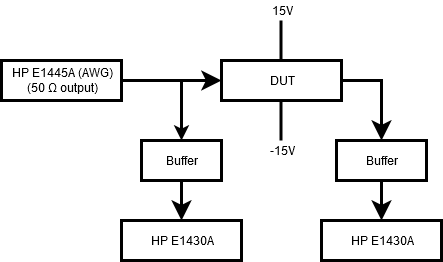
\includegraphics[width = 0.6\textwidth]{figures/DUT_setup.png}
    \caption{Diagram of the measurement set-up}
    \label{fig:set-up}
\end{figure}

\newpage
\subsection{Nonparametric estimate}
\label{sec:nonparametric_estimate_controller}
The first step in this experiment is to get a nonparametric estimate of the FRF of the system $G(s)$. However, the Wiener-Hammerstein system is nonlinear. This means that the system cannot be represented by a TF. However, we can find the best linear approximation (BLA) of the system $G_{\textrm{BLA}}$. With an intelligently designed excitation signal, it is possible to suppress the non-linearities in the input and output signals \cite{pintelon_book}. Neglecting the transient term, we can say that the output spectrum contains 3 contributions if it is excited by an input $U(k)$:
\begin{itemize}
	\item A linear contribution from $G_{\textrm{BLA}}(\Omega_k) U(k)$
	\item A random noise contribution that doesn't depend on the input $N_Y(k)$
	\item A nonlinear distortion term that does depend on the input $Y_S(k)$
\end{itemize}
Thus, we can write
\begin{equation*}
	Y(k) = G_{\textrm{BLA}}(\Omega_k) U(k) + N_Y(k) + Y_S(k)
\end{equation*}
If we apply the input for $P$ periods we get
\begin{equation*}
	Y^{(p)}(k) = G_{\textrm{BLA}}(\Omega_k) U(k) + N_Y^{(p)}(k) + Y_S(k) \,, \quad p = 1,\ldots,P
\end{equation*}
Only the random noise contribution differs from period to period. As the nonlinear distortions depend on the input, they will be the same for every period. In this way, we are blind to the nonlinear distortions. They will remain in our estimate of the best linear approximation $\hat G_{\textrm{BLA}}$ even if we apply the excitation signal for an infinite amount of periods.

The solution to this problem is to design $M$ realizations of the excitation signal. More specifically, in the case of multisine excitations, this means that multiple multisines must be designed with different random phases for every excited harmonic. The amplitude of the sine components can be the same for every realization.
\begin{equation*}
	U^{(m)}(k) = A_k e^{j \phi_k^{(m)}} \,, \quad \phi_k^{(m)} \sim \mathcal{U}(0,2\pi) \,, \quad m = 1,\ldots,M
\end{equation*}
These $M$ different realizations can be applied for $P$ periods. The output spectrum for the $p$-th period of the $m$-th realization is then given by
\begin{equation*}
	Y^{(m,p)}(k) = G_{\textrm{BLA}}(\Omega_k) U^{(m)}(k) + N_Y^{(m,p)}(k) + Y_S^{(m)}(k) 
\end{equation*}
The random noise contribution is different for every period of every realization. The nonlinear distortions are different for every realization. Dividing the output spectrum by the input spectrum gives us a nonparametric estimate of the FRF of $G_{\textrm{BLA}}$ for every period of every realization.
\begin{equation*}
	\hat G^{(m,p)}(\Omega_k) = \frac{Y^{(m,p)}(k)}{U^{(m)}(k)} = G_{\textrm{BLA}}(\Omega_k)  + \frac{N_Y^{(m,p)}(k)}{U^{(m)}(k)} + \frac{Y_S^{(m)}(k)}{U^{(m)}(k)}
\end{equation*}
Now, as a result of applying multiple realizations of the input signal, the nonlinear distortions can be isolated from the linear contributions and suppressed. This results in a better estimate of the FRF of the best linear approximation. 

More information on how to estimate the FRF of the best linear approximation can be found in \cite[Chapter 4]{pintelon_book}. With that said, a multisine was applied to the \mbox{Wiener-Hammerstein} system by using the measurement set-up shown in figure \ref{fig:set-up}. 

\newpage
The excitation signal had the following properties:
\begin{itemize}
\item Sampling frequency: $f_s = 78.125 \,\textrm{kHz}$
\item Samples per period: $N = 2048$
\item Periods per realization: $P = 2$
\item Number of realizations: $M = 20$
\item Excited harmonics: $\kexc = \{k \in \mathbb{N} : 1 \leq k \leq 262\}$
\item Input RMS: $V_{\mathrm{RMS}} = 100 \, \textrm{mV}$
\item Sine component amplitude: $A_k^{(1)} = \ldots = A_k^{(M)} = \text{constant} \,, \quad \forall k \in \kexc$
\item Sine component phases: $\phi_k^{(m)} \sim \mathcal{U}(0,2\pi) \,, \quad m = 1, \ldots, M \,, \quad \forall k \in \kexc$ 
\end{itemize}
The 262-nd harmonic corresponds to the maximum excited frequency
\begin{equation*}
	f_{\mathrm{max}} = 262 \frac{f_s}{N} = 9994.5 \, \mathrm{Hz} \approx 10 \,\textrm{kHz}
\end{equation*}

The measurement set-up automatically waits for the system to be in steady state before taking measurements. However, noise transients can still be present in the input and output spectra. Therefore, the Robust LPM is used to obtain a nonparametric estimate of the FRF of the system at the excited frequencies. Additionally, because multiple realizations are measured, the Robust LPM can discern between the noise variance and the nonlinear distortions. 

Using the heuristics mentioned in section \ref{sec:choice_order_dof}, the order and degrees of freedom best suitable for the Robust LPM can be determined. After applying the Robust LPM for different values of the order and the degrees of freedom, it was observed that increasing either of these parameters doesn't decrease the total estimated variance of the FRF. Thus the default parameters $R=2$ and $q^{\mathrm{noise}}=1$ are used. The nonparametric estimate of the FRF of the best linear approximation of the Wiener-Hammerstein system is shown in figure \ref{fig:GBLA_nonparam}. The nonlinear distortion are clearly dominant over the random noise contributions. This is the reason why $M=20$ realizations were measured.

\begin{figure}[H]
\centering
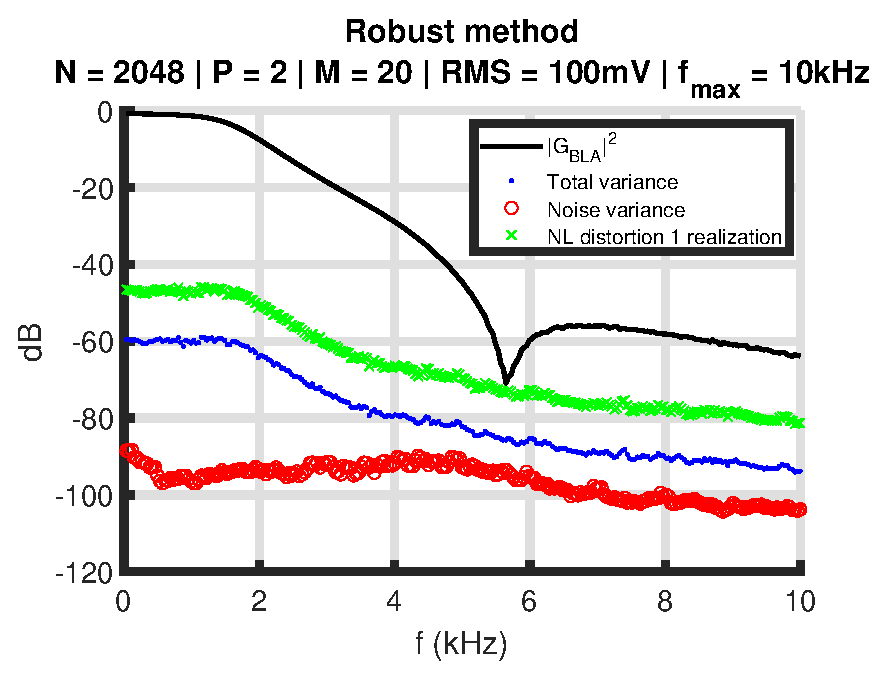
\includegraphics[width = 0.65\textwidth]{figures/robust_method_G.eps}
\caption{Nonparametric estimate of the FRF of the best linear approximation of the Wiener-Hammerstein system.}
\label{fig:GBLA_nonparam}
\end{figure}

\subsection{Controller design}
\label{sec:controller_design_controller}
Now that we have a nonparametric estimate of the FRF of $G_{\textrm{BLA}}(s)$, we can design an analog controller for it.

After experimenting with multiple reference models $M(s)$ and controller structures $K(s,\rho)$, the following resulted in a suitable closed loop system.
\begin{align*}
&M(s) = M_1(s) M_2(s) \\
\text{with } &M_1(s) = \frac{\omega_1^2}{s^2 + 2\omega_1s + \omega_1^2} \,, \quad \omega_1 = 2 \pi \, 5000 \, \mathrm{Hz} \\
\text{and } &M_2(s) = \frac{\omega_2^2}{s^2 + 2\omega_2s + \omega_2^2} \,, \quad \omega_2 = 2 \pi \, 8000 \, \mathrm{Hz} \\
&K(s,\rho) = \rho_0 + \frac{\rho_1}{s} + \rho_2 s + \rho_3 s^2
\end{align*}
Additionally, the optimization ignores the frequencies larger than $4 \, \mathrm{kHz}$.
\begin{equation*}
	F(j \omega) = \begin{cases}
		1 & \text{if } |\omega| \leq 2\pi \, 4 \, \mathrm{kHz} \\
		0 & \text{if } |\omega| > 2\pi \, 4 \, \mathrm{kHz}
	\end{cases}
\end{equation*}
This was done because there is a transmission zero between $5 \, \mathrm{kHz}$ and $6 \, \mathrm{kHz}$ (figure \ref{fig:GBLA_nonparam}). The gain of the controller would need to be infinite at that frequency in order to compensate for this.

The FD cost function (\ref{eq:JFD}) was optimized without any constraints. The optimal parameters are

\begin{equation*} \rho_{\mathrm{opt}} = 
\begin{bmatrix}
\rho_0\\\rho_1\\\rho_2\\\rho_3
\end{bmatrix} = 
\begin{bmatrix}
2.580\\4533 \, \textrm{sec}^{-1}\\1.443 . 10^{-3} \, \textrm{sec}\\1.775 . 10^{-8} \, \textrm{sec}^{2}
\end{bmatrix}
\end{equation*}
The closed loop system that would result from this controller can then be determined nonparametrically using
\begin{equation}
	\mathrm{CL}(j\omega_k) = \frac{K(j\omega_k, \rho_{\mathrm{opt}}) \hat G_{\mathrm{BLA}}(j\omega_k)}{1 + K(j\omega_k, \rho_{\mathrm{opt}}) \hat G_{\mathrm{BLA}}(j\omega_k)}
	\label{eq:optimal_CL}
\end{equation}
The resulting closed loop system is shown in figure \ref{fig:GBLA_M_CL_nonparam}. The proposed controller structure $K(s,\rho)$ cannot realize the reference model $M(s)$ perfectly. However, the optimal closed loop system $\mathrm{CL}(s)$ remains close to the reference model until $4 \, \mathrm{kHz}$. 

\begin{figure}[H]
\centering
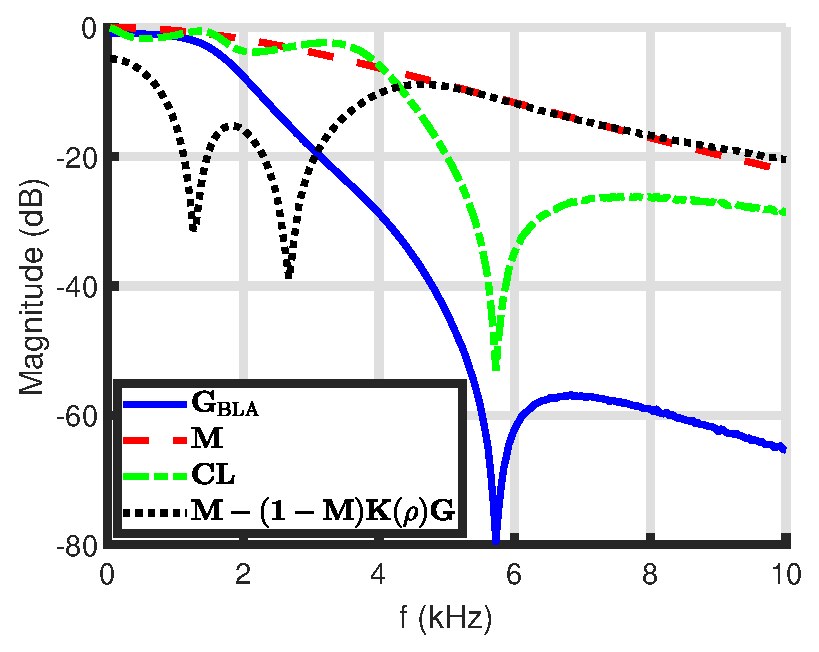
\includegraphics[width = 0.65\textwidth]{figures/real_system_nonparametric_closed_loop.eps}
\caption{Nonparametric estimates of the FRF of $G_{\mathrm{BLA}}(s)$, the reference model $M(s)$, the closed loop system $\mathrm{CL}(s)$ and the stability criteria $[M - (1-M)K(\rho_{\mathrm{opt}})G]$.}
\label{fig:GBLA_M_CL_nonparam}
\end{figure}

Additionally, the stability criteria $[M - (1-M)K(\rho_{\mathrm{opt}})G]$ are also plotted in figure \ref{fig:GBLA_M_CL_nonparam}. This quantity is below 1 in amplitude (0 dB) for all excited harmonics $\kexc$, which means that the stability of the closed loop system might be guaranteed. To guarantee the stability of the closed loop system, the system $G_{\mathrm{BLA}}$ must be stable. This is the case. Moreover, $\frac{M(s)}{1-M(s)}$ must also be stable. The poles of $\frac{M(s)}{1-M(s)}$ are shown in figure \ref{fig:M_one_minus_M_poles}. None of the poles are in the right half plane, which means that $\frac{M(s)}{1-M(s)}$ is stable. Finally, we have only shown that $[M - (1-M)K(\rho_{\mathrm{opt}})G]$ is below 1 in amplitude for the excited frequencies. Therefore, we must also assume that the frequency resolution $f_s/N$ is high enough to ensure that no resonance peaks are missed. We must also assume that $[M - (1-M)K(\rho_{\mathrm{opt}})G]$ remains below 1 in amplitude for $f > 10 \, \mathrm{kHz}$. Assuming these things, the stability of the closed loop system is guaranteed.

\begin{figure}[H]
\centering
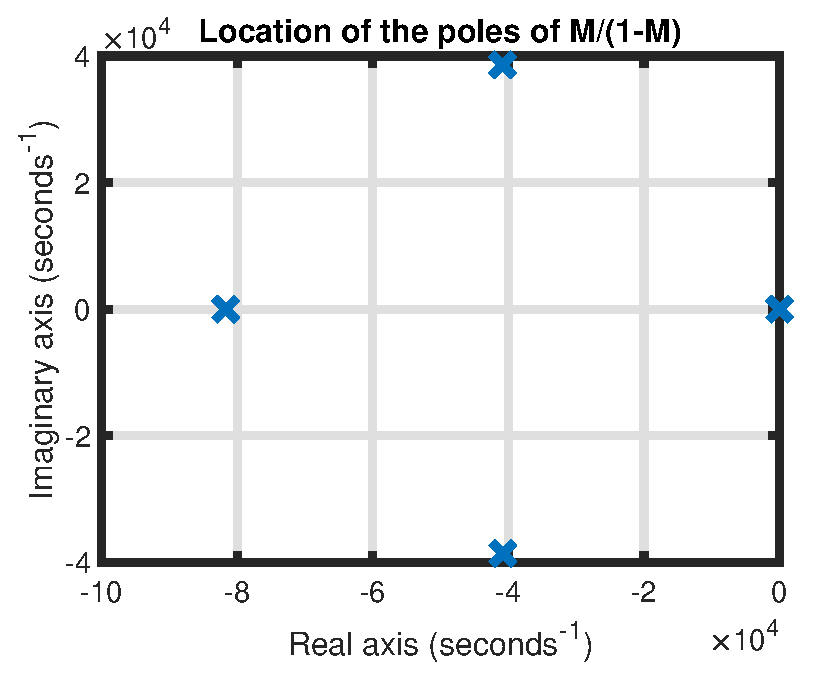
\includegraphics[width = 0.65\textwidth]{figures/M_one_minus_M_poles.eps}
\caption{Location of the poles of $\frac{M(s)}{1-M(s)}$}
\label{fig:M_one_minus_M_poles}
\end{figure}

\subsection{Controller realization}
The analog controller is built using TL074 operational amplifiers (OPAMP). The schematic is shown in figure \ref{fig:controller_schematic}. The capacitor in the integrator has a resistor
in parallel in order to limit the DC gain of the integrator. Extra components were also added to the second differentiator to limit the high-frequency (HF) gain as it was observed experimentally that the output of the second differentiator was very noisy without those components.

\begin{figure}[p]
	\centering
    
\includegraphics[angle=90,height=\textheight]{figures/circuit_annotated.jpg}
    \caption{Schematic of the controller.}
    \label{fig:controller_schematic}
\end{figure}

The controller was simulated in LTspice XVII.\footnote{\url{https://www.analog.com/en/design-center/design-tools-and-calculators/ltspice-simulator.html} (visited on 3 August 2020)} The FRF of the simulated analog controller is compared to the optimal controller $K(\rho_{\mathrm{opt}})$ in figure \ref{fig:controller_simulation}. The red dotted line shows the FRF of the simulated controller if no extra resitor and capacitor are added to the second differentiator. The gain almost reaches 120 dB. However, in this case, the HF gain still goes to zero due to the limitations of the TL074 OPAMPs. The blue dash-dotted line shows the simulated controller with the components added to the second differentiator. The maximal gain decreases significantly. Finally, the discrepancy in the low frequencies is due to the finite DC gain of the integrator. In the frequency range of interest, which is between 10 Hz and 10 kHz, the difference between the optimal controller and the simulated controller is not very significant.


\begin{figure}[H]
\centering
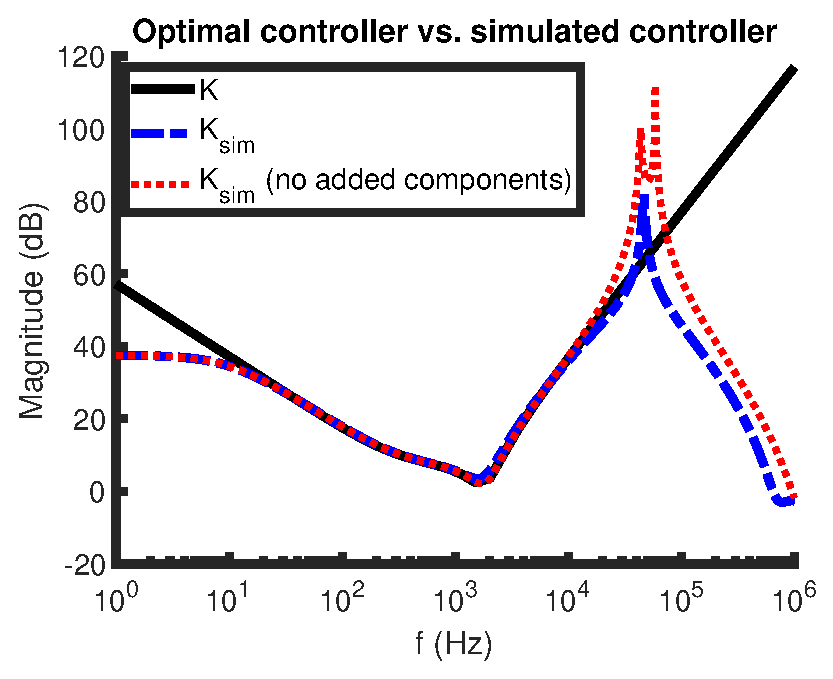
\includegraphics[width = 0.65\textwidth]{figures/controller_simulation.eps}
\caption{Optimal controller $K(\rho_\mathrm{opt})$ vs. the simulated controller from figure \ref{fig:controller_schematic}, with and without added resistor and capacitor to the second differentiator.}
\label{fig:controller_simulation}
\end{figure}


\newpage
The controller was soldered on a stripboard. The realized controller is shown in figure \ref{fig:controller_real}.

\begin{figure}
\centering
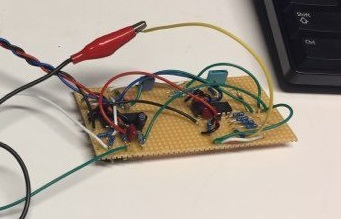
\includegraphics[width = 0.65\textwidth]{figures/controller_real.jpg}
\caption{Built controller.}
\label{fig:controller_real}
\end{figure}


The controller was measured with the measurement set-up (figure \ref{fig:set-up}). The excitation has the same properties as the excitation signal in section \ref{sec:nonparametric_estimate_controller}, except for one thing: the sine component amplitude is not flat. The amplitudes $A_k$ were shaped such that the energy is high at frequencies where the gain is expected to be low. The amplitudes are inversely proportional to the magnitude of the optimal controller $K(\rho_{\mathrm{opt}})$. The energy of the signal is also different. It is now $29.3 \, \mathrm{mV}_\mathrm{RMS}$. The amplitude spectrum of the input excitation used to measure the controller is shown in figure \ref{fig:controller_input_for_meas}.


\begin{figure}[H]
\centering
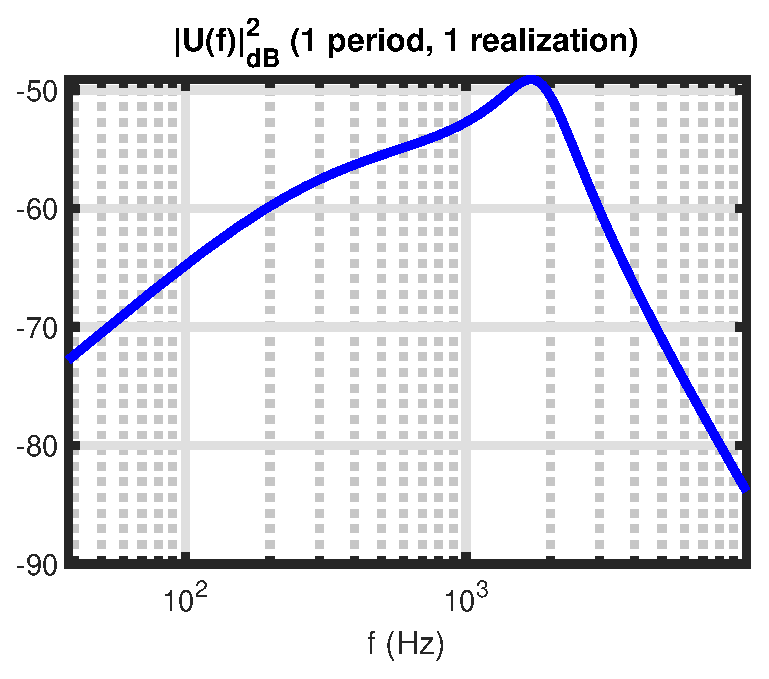
\includegraphics[width = 0.65\textwidth]{figures/controller_input_for_meas.eps}
\caption{Amplitude spectrum of one period of one realization of the input excitation used to measure the controller.}
\label{fig:controller_input_for_meas}
\end{figure}

\newpage
The nonparametric estimate of the FRF of the analog controller is shown in figure \ref{fig:controller_nonparam_measure}. The realized controller does not conform to the optimal controller $K(s,\rho_{\mathrm{opt}})$. However, as will be explained further, we believe these measurements to be invalid.

\begin{figure}[H]
\centering
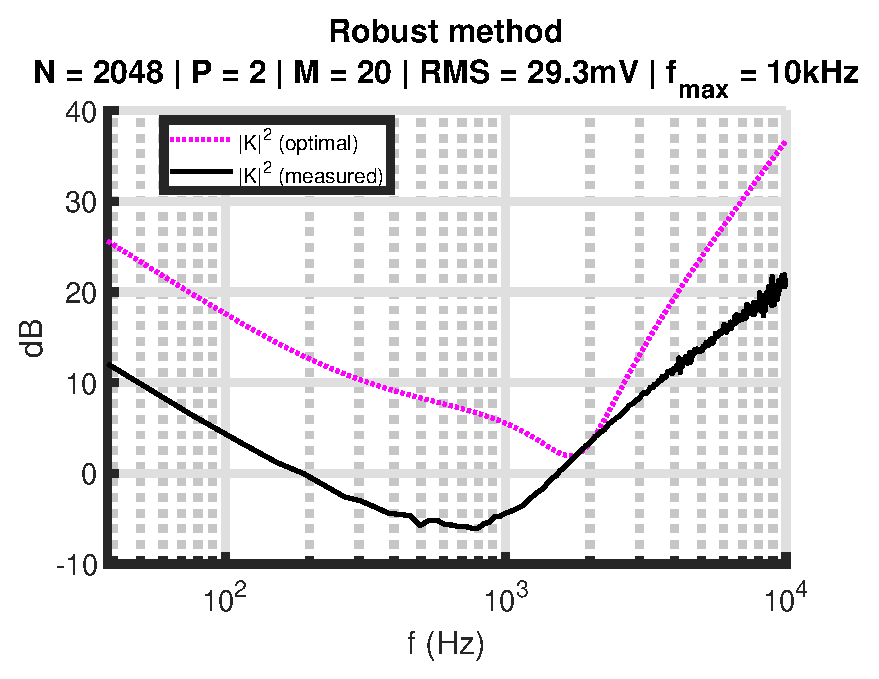
\includegraphics[width = 0.65\textwidth]{figures/robust_method_K.eps}
\caption{Nonparametric estimate of the FRF of the analog controller.}
\label{fig:controller_nonparam_measure}
\end{figure}

\newpage
\subsection{Closed loop}
Next, the Wiener-Hammerstein system was connected to the controller in closed loop with unity negative feedback (figure \ref{fig:closed_loop_system}). The same properties of the excitation signal that were used in sections \ref{sec:nonparametric_estimate_controller} and \ref{sec:controller_design_controller} are used here. One exception is the shape of the amplitude spectrum $A_k$. The best linear approximation of the Wiener-Hammerstein system depends on the energy of the input to that system as it is nonlinear. The reference signal was shaped in order to make sure that the input to the system is close to flat with an energy of $100 \, \mathrm{mV}_\mathrm{RMS}$. Now the amplitude spectrum of the reference signal is inversely proportional to the magnitude of the TF between the reference and the input to the system, which is $\frac{\hat G_{\mathrm{BLA}}(j \omega_k)}{1+K(j \omega_k,\rho_\mathrm{opt}) \hat G_{\mathrm{BLA}}(j \omega_k)}$. This also changes the energy of the reference signal. It is now $42.9 \, \mathrm{mV}_\mathrm{RMS}$. The resulting nonparametric estimate of the FRF of the closed loop system is shown in figure \ref{fig:CL_measure}. The result is quite close to the optimal closed loop FRF (\ref{eq:optimal_CL}). Moreover, the closed loop system is stable.

\begin{figure}[H]
\centering
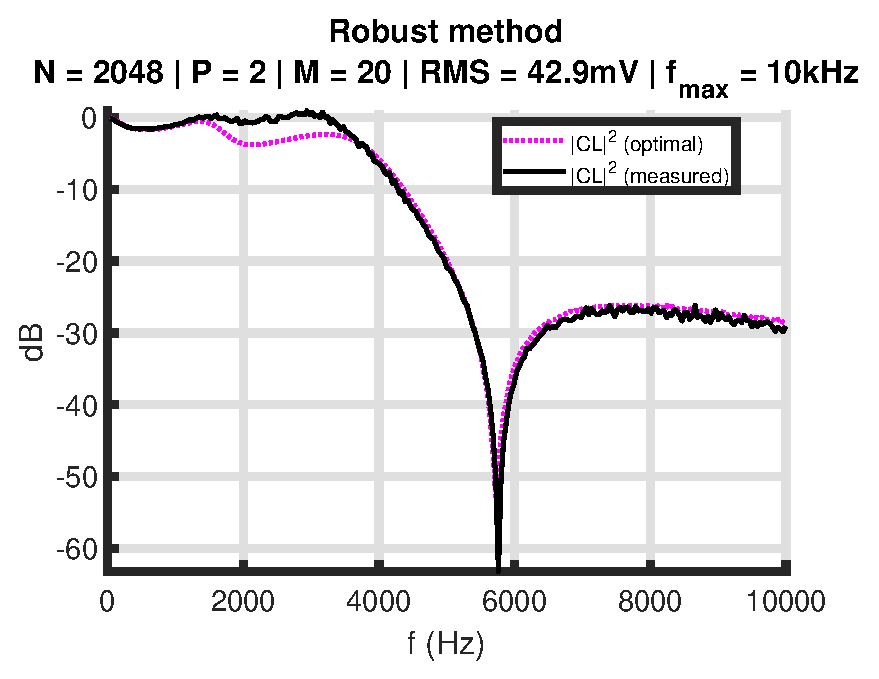
\includegraphics[width = 0.65\textwidth]{figures/robust_method_CL.eps}
\caption{Nonparametric estimate of the FRF of the closed loop system.}
\label{fig:CL_measure}
\end{figure}

\newpage
The success of the measurement of the closed loop system suggests that the nonparametric estimate of the FRF of the analog controller is invalid. We can estimate the FRF of the analog controller indirectly from the estimated closed loop FRF $\hat{\textrm{CL}}(j\omega_k)$ and the estimated FRF of the best linear approximation of the system $\hat G_{\mathrm{BLA}}(j\omega_k)$.
\begin{equation*}
	\hat{K}_{\mathrm{indirect}}(j\omega_k) =  \frac{\hat{\textrm{CL}}(j\omega_k)}{\hat G_{\mathrm{BLA}}(j\omega_k)(1-\hat{\textrm{CL}}(j\omega_k))}
\end{equation*}
The indirect estimate of the FRF of the controller is shown in figure \ref{fig:K_from_G_CL}. The controller is very close to the optimal controller. The indirect estimate spikes around $5.6 \, \mathrm{kHz}$, but this is just because the FRF of the system and the FRF of the closed loop system are zero around that frequency, which results in a division of zero by zero.

\begin{figure}[H]
\centering
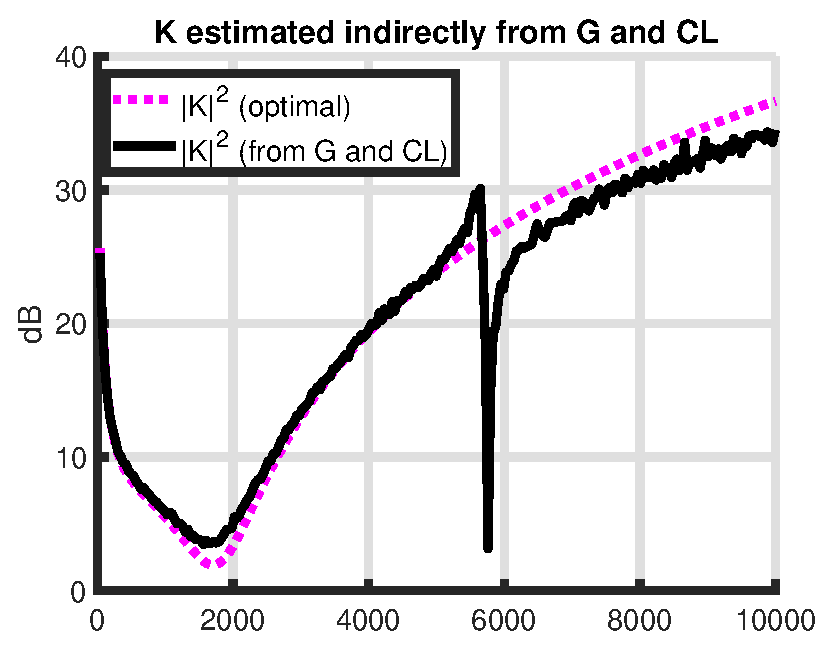
\includegraphics[width = 0.65\textwidth]{figures/K_from_G_CL.eps}
\caption{Indirect estimate of the FRF of the controller from $\hat{\textrm{CL}}(j\omega_k)$ and $G_{\mathrm{BLA}}(j\omega_k)$.}
\label{fig:K_from_G_CL}
\end{figure}

\section{Conclusion}
The FD method was used to design an analog controller for a Wiener-Hammerstein system. The stability constraints were used to guarantee the stability of the closed loop system. Then, the analog controller was constructed successfully. Finally, the analog controller and closed loop system were measured. However, the measurement of the analog controller was not successful. The cause of this failure is unknown.